% Anexos complementarios del Manual de Usuario.
% Este archivo se incluye desde manual_usuario.tex y conserva la numeración A.
% Las figuras son material de consulta adicional; las pantallas principales permanecen junto a sus procedimientos.

\subsubsection{Anexo A.1. Catálogo visual de componentes}
La siguiente lámina reúne componentes visuales que aparecen en más de un módulo. Su finalidad es facilitar la identificación de campos, botones, listas desplegables, formularios y acciones contables antes de operar el sistema.

\begin{figure}[H]
    \centering
    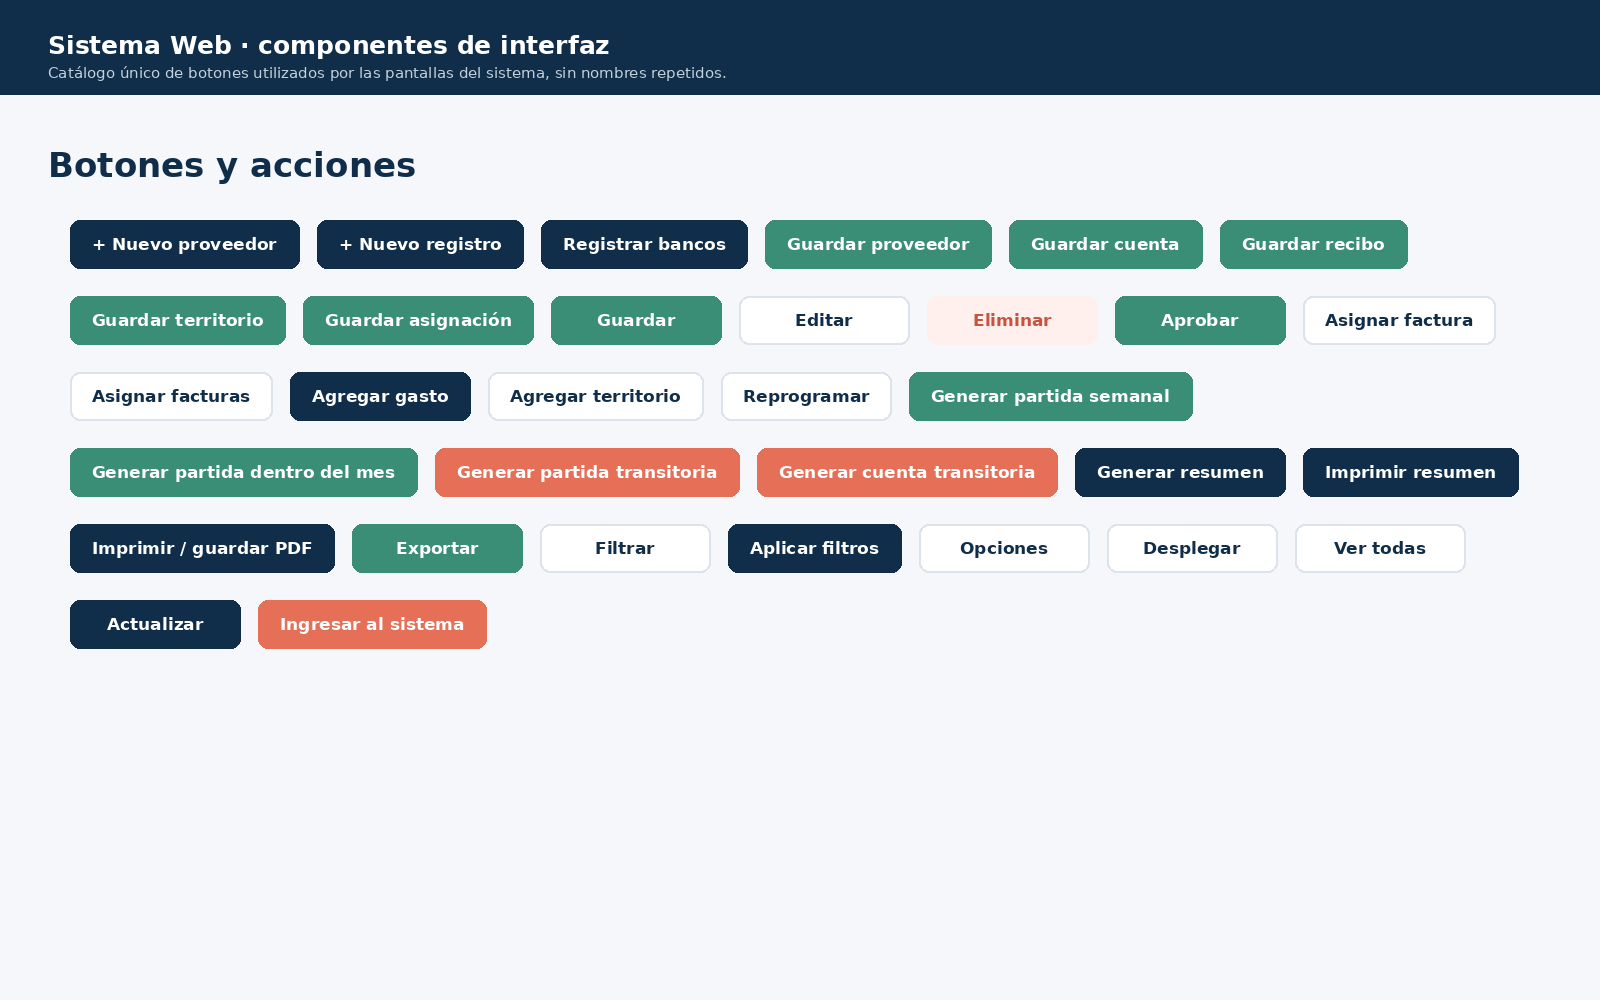
\includegraphics[width=0.88\textwidth]{imagenes/elementos_01_botones.png}
    \caption{Botones y acciones de uso frecuente}
    \label{fig:A_componentes_botones}
\end{figure}

\begin{figure}[H]
    \centering
    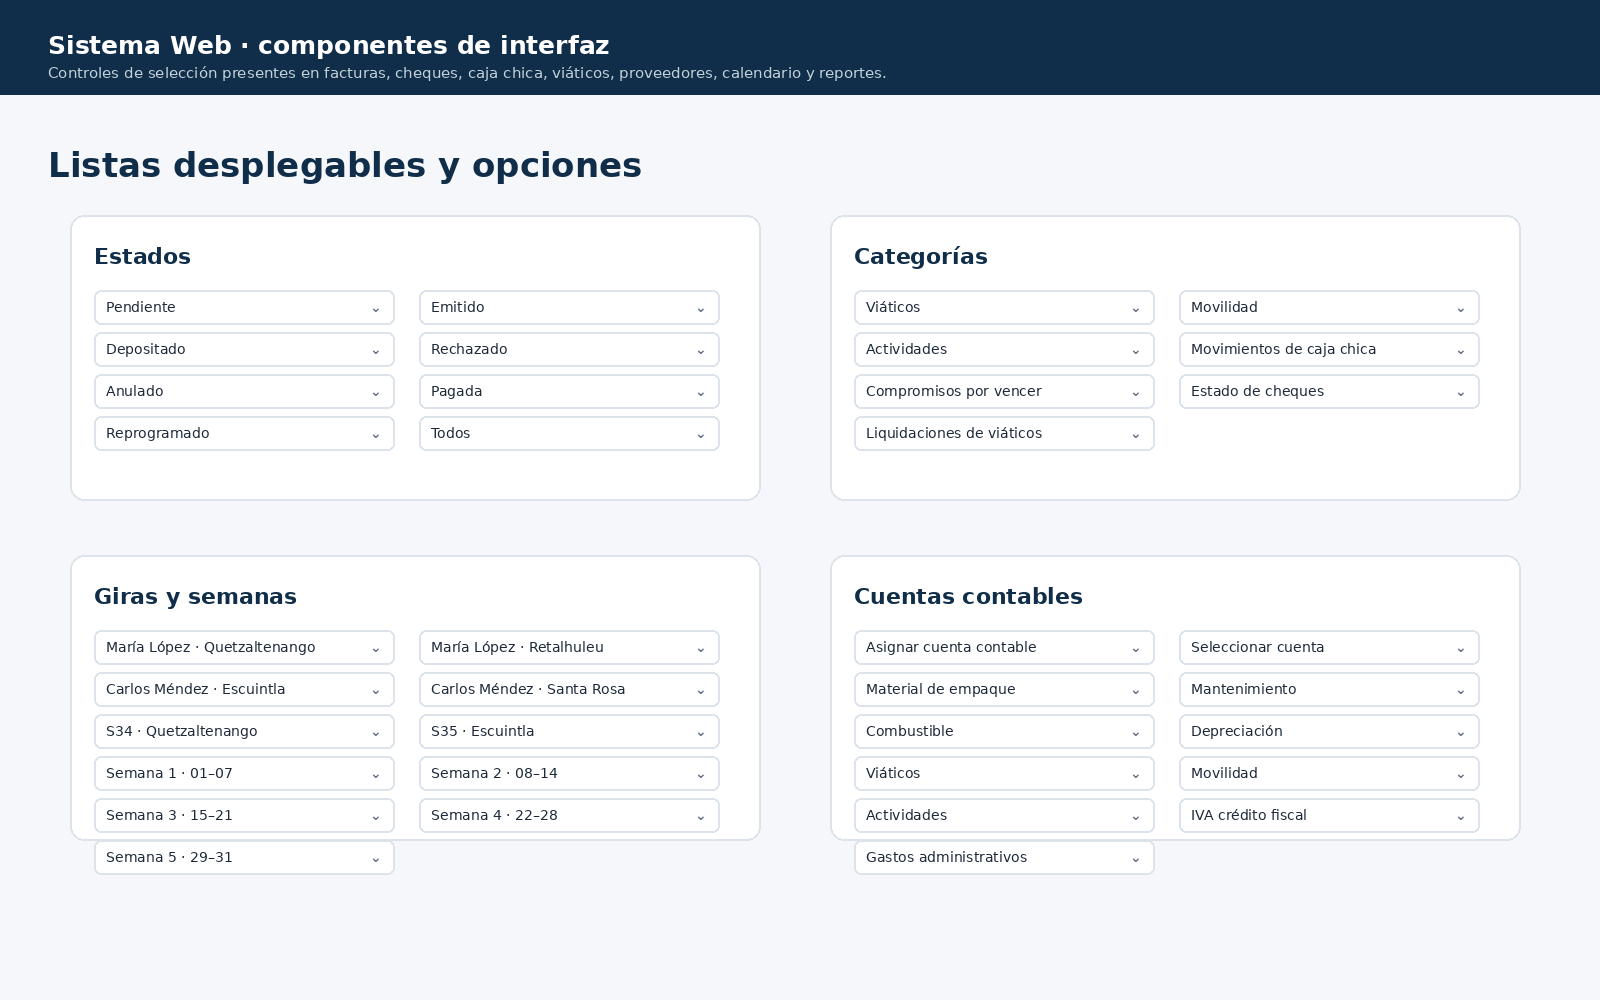
\includegraphics[width=0.88\textwidth]{imagenes/elementos_02_listas_desplegables.png}
    \caption{Listas desplegables y selección de opciones}
    \label{fig:A_componentes_listas}
\end{figure}

\begin{figure}[H]
    \centering
    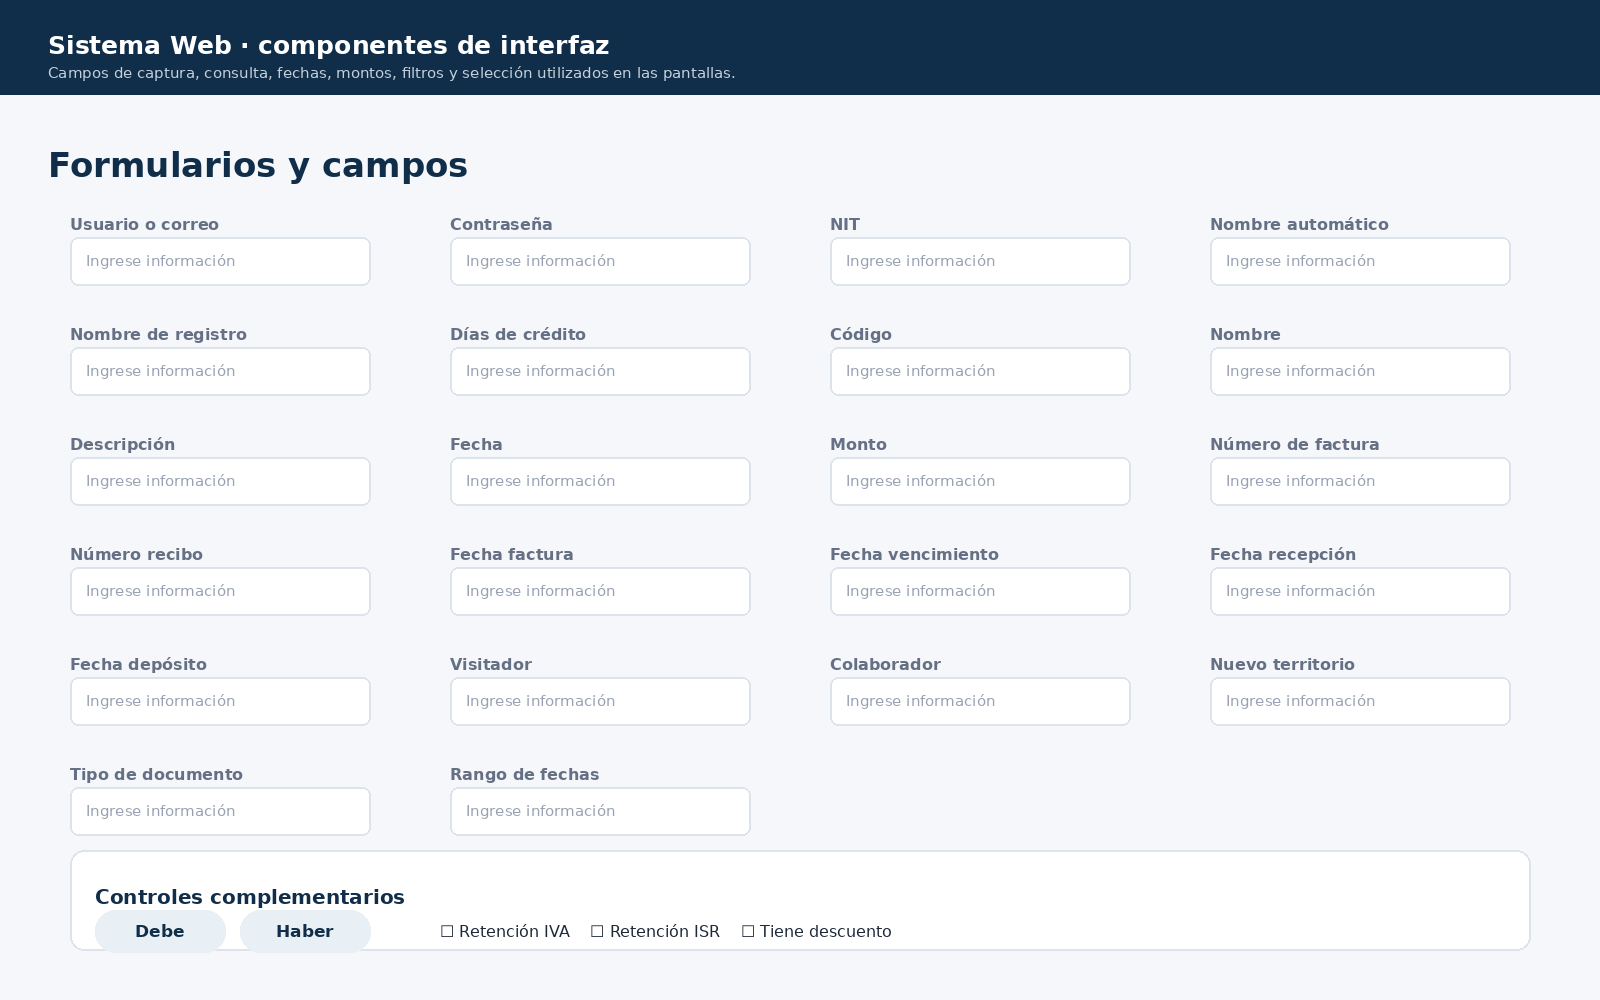
\includegraphics[width=0.88\textwidth]{imagenes/elementos_03_formularios.png}
    \caption{Campos y formularios de registro}
    \label{fig:A_componentes_formularios}
\end{figure}

\begin{figure}[H]
    \centering
    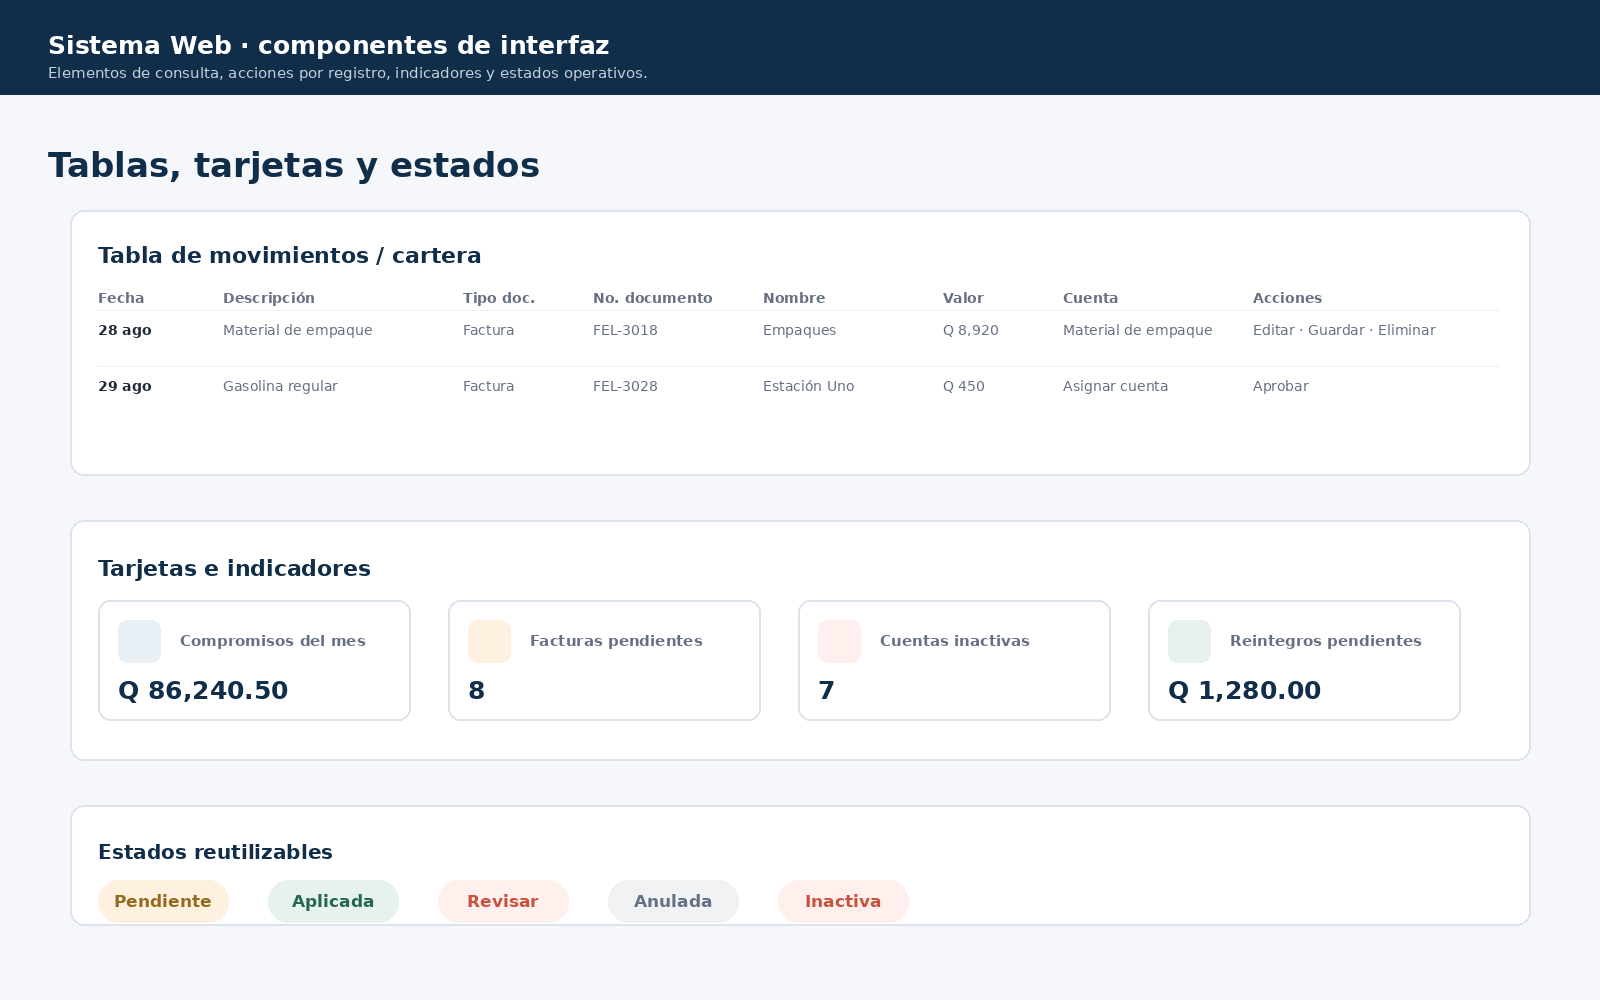
\includegraphics[width=0.88\textwidth]{imagenes/elementos_04_tablas_tarjetas.png}
    \caption{Tablas, tarjetas y agrupación de información}
    \label{fig:A_componentes_tablas}
\end{figure}

\begin{figure}[H]
    \centering
    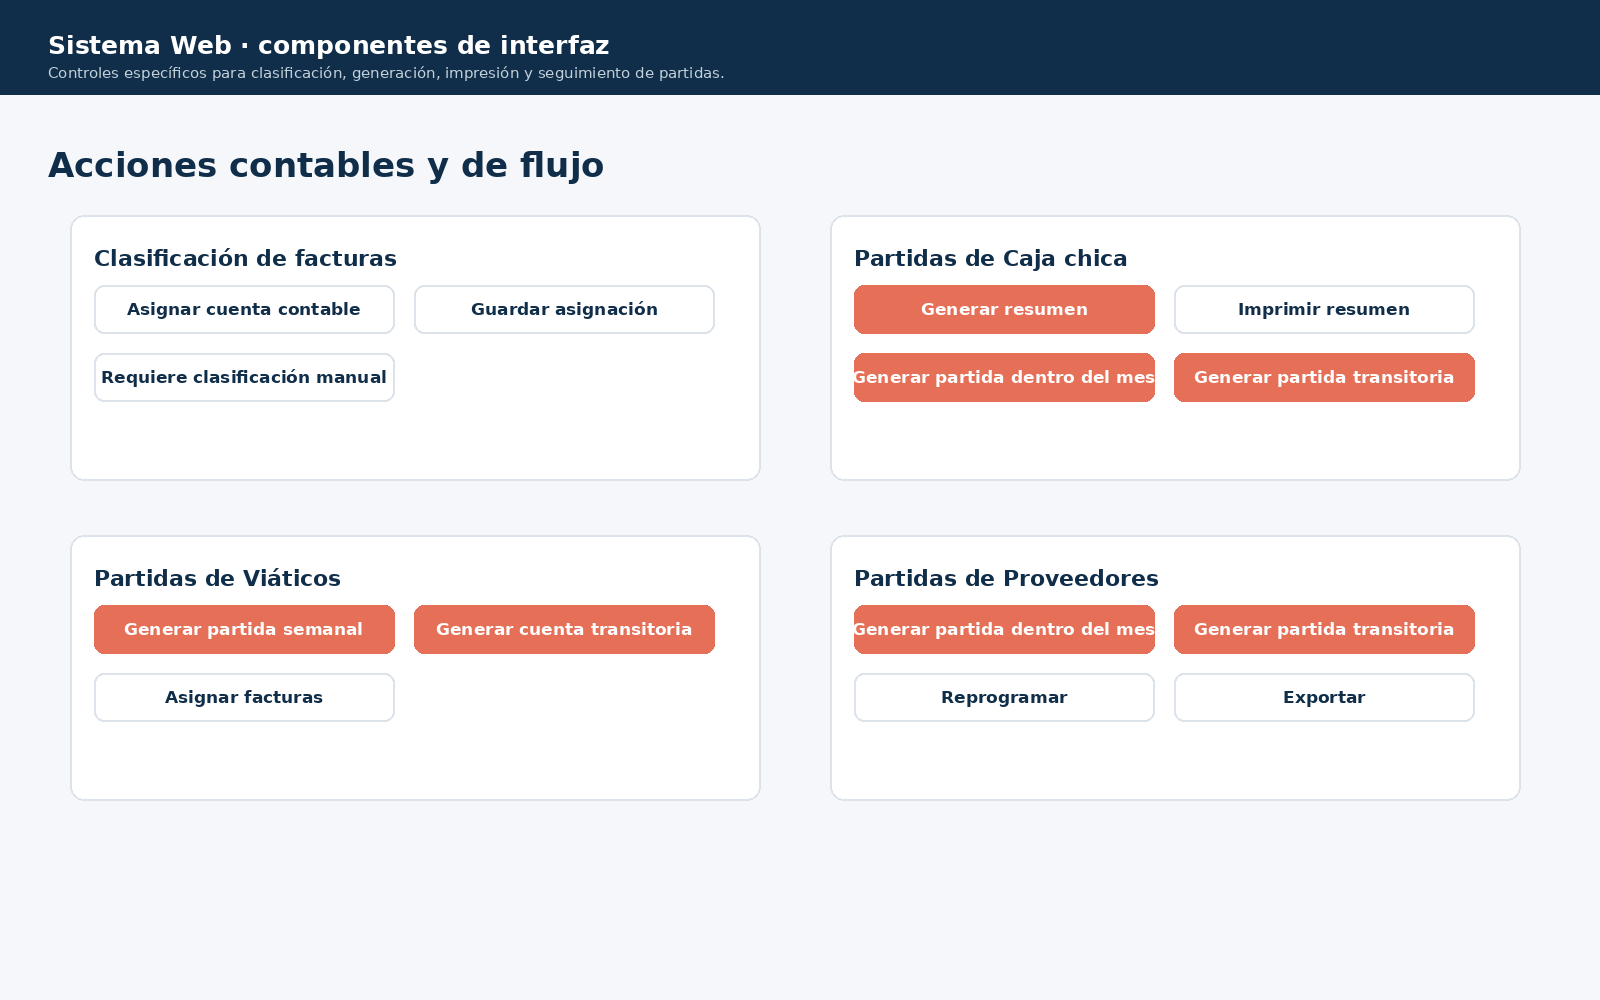
\includegraphics[width=0.88\textwidth]{imagenes/elementos_05_acciones_contables.png}
    \caption{Acciones relacionadas con registros contables}
    \label{fig:A_componentes_contables}
\end{figure}

\subsubsection{Anexo A.2. Inventario de pantallas y propósito operativo}
La Tabla~\ref{tab:A_inventario_pantallas} resume las pantallas documentadas y su propósito principal. El inventario sirve como referencia rápida y no sustituye los procedimientos explicados en el cuerpo del manual.

\begin{longtable}{p{1.1cm}p{4.0cm}p{8.1cm}}
\caption{Inventario de pantallas del sistema}\label{tab:A_inventario_pantallas}\\
\toprule
\textbf{No.} & \textbf{Pantalla} & \textbf{Propósito operativo}\\
\midrule
01 & Login & Autenticar al usuario y permitir el ingreso seguro al sistema.\\
02 & Panel principal & Consultar los módulos disponibles y el resumen de operaciones.\\
03 & Facturas FEL/SAT & Consultar, importar y validar facturas electrónicas.\\
04 & Cheques posfechados & Registrar cheques, bancos, fechas, estados y asignaciones.\\
05 & Caja chica & Registrar movimientos, documentos, cuentas y resumen del período.\\
06 & Viáticos & Gestionar colaboradores, territorios, giras, categorías y partidas.\\
07 & Asignación de facturas & Asociar facturas con colaboradores, giras y cuentas contables.\\
08 & Proveedores & Registrar proveedores, condiciones de crédito y cartera.\\
09 & Calendario operativo & Consultar fechas y actividades relevantes de la operación.\\
10 & Nomenclatura contable & Registrar cuentas contables, naturaleza y estado.\\
11 & Reportes & Consultar reportes autorizados del sistema.\\
12 & Resumen de Caja chica & Revisar e imprimir el resumen de movimientos del período.\\
\bottomrule
\end{longtable}

\subsubsection{Anexo A.3. Lista de verificación para el usuario}
Antes de cerrar una operación, el usuario puede utilizar la siguiente lista de verificación. Las casillas se dejan sin marcar para que puedan emplearse como instrumento de consulta o imprimirse según las necesidades de la organización.

\begin{longtable}{p{0.9cm}p{9.5cm}p{3.0cm}}
\caption{Lista de verificación operativa del usuario}\label{tab:A_checklist_usuario}\\
\toprule
\textbf{No.} & \textbf{Verificación} & \textbf{Estado}\\
\midrule
1 & Se ingresó con las credenciales asignadas al usuario. & \rule{2.5cm}{0.4pt}\\
2 & Se revisó el Panel principal antes de iniciar el período. & \rule{2.5cm}{0.4pt}\\
3 & Las facturas FEL/SAT fueron consultadas o importadas sin duplicados. & \rule{2.5cm}{0.4pt}\\
4 & Las facturas no reconocidas tienen cuenta de nomenclatura asignada. & \rule{2.5cm}{0.4pt}\\
5 & Los movimientos de Caja chica contienen documento, valor y cuenta contable. & \rule{2.5cm}{0.4pt}\\
6 & Las liquidaciones de Viáticos tienen colaborador, gira, territorio y semana. & \rule{2.5cm}{0.4pt}\\
7 & Los proveedores tienen datos de registro, crédito y retenciones revisados. & \rule{2.5cm}{0.4pt}\\
8 & Las partidas muestran igualdad entre Debe y Haber antes de guardarse. & \rule{2.5cm}{0.4pt}\\
9 & Se generó y resguardó el reporte autorizado del período. & \rule{2.5cm}{0.4pt}\\
\bottomrule
\end{longtable}

\subsubsection{Anexo A.4. Criterios para reportar incidencias}
Cuando una operación no produzca el resultado esperado, registre la fecha, el módulo, la acción realizada, el mensaje mostrado y una captura de la pantalla. No comparta contraseñas ni información sensible en el reporte. La incidencia debe remitirse al responsable designado con los datos suficientes para reproducir el problema.
